\documentclass{article}

\usepackage[letterpaper, portrait, margin=1.5in]{geometry}

\usepackage{fancyhdr}
\usepackage{ragged2e}
\usepackage{graphicx}
\usepackage{caption}
\usepackage{amsmath}
\usepackage{rotating}

\usepackage{listings}
\usepackage{color}

\definecolor{dkgreen}{rgb}{0,0.6,0}
\definecolor{gray}{rgb}{0.5,0.5,0.5}
\definecolor{mauve}{rgb}{0.58,0,0.82}

\lstset{frame=tb,
  language=Java,
  aboveskip=3mm,
  belowskip=3mm,
  showstringspaces=false,
  columns=flexible,
  basicstyle={\small\ttfamily},
  numbers=none,
  numberstyle=\tiny\color{gray},
  keywordstyle=\color{blue},
  commentstyle=\color{dkgreen},
  stringstyle=\color{mauve},
  breaklines=true,
  breakatwhitespace=true,
  tabsize=4
}

\setcounter{secnumdepth}{1}

\usepackage{chngcntr}
\counterwithin{figure}{section}

\renewcommand*{\thepage}{C\arabic{page}}

\pagestyle{fancy}
\lhead{ACME Robotics}
\chead{\#8367}
\rhead{\ifcontents Contents \else Week \thesection \fi}

\newif\ifcontents
\contentstrue

\makeatletter
\renewcommand{\@seccntformat}[1]{}
\makeatother
\begin{document}

\subsection{Drive Practice}
%! Run matches with the drive team. 
Over the week, the drive team ran practice matches to practice their driving skills. The drive team consists of Shawn and Aidan as the drivers and Emma as the drive coach. At the beginning of the week, they just ran the teleop part of a match, using a real FTC timer that they found on YouTube. They kept track of their scores and performance on the whiteboard, as seen in fig \ref{fig:chart}. For their first round of drive practice, they were averaging about 120 points during just teleop. 

\begin{figure}
    \centering
    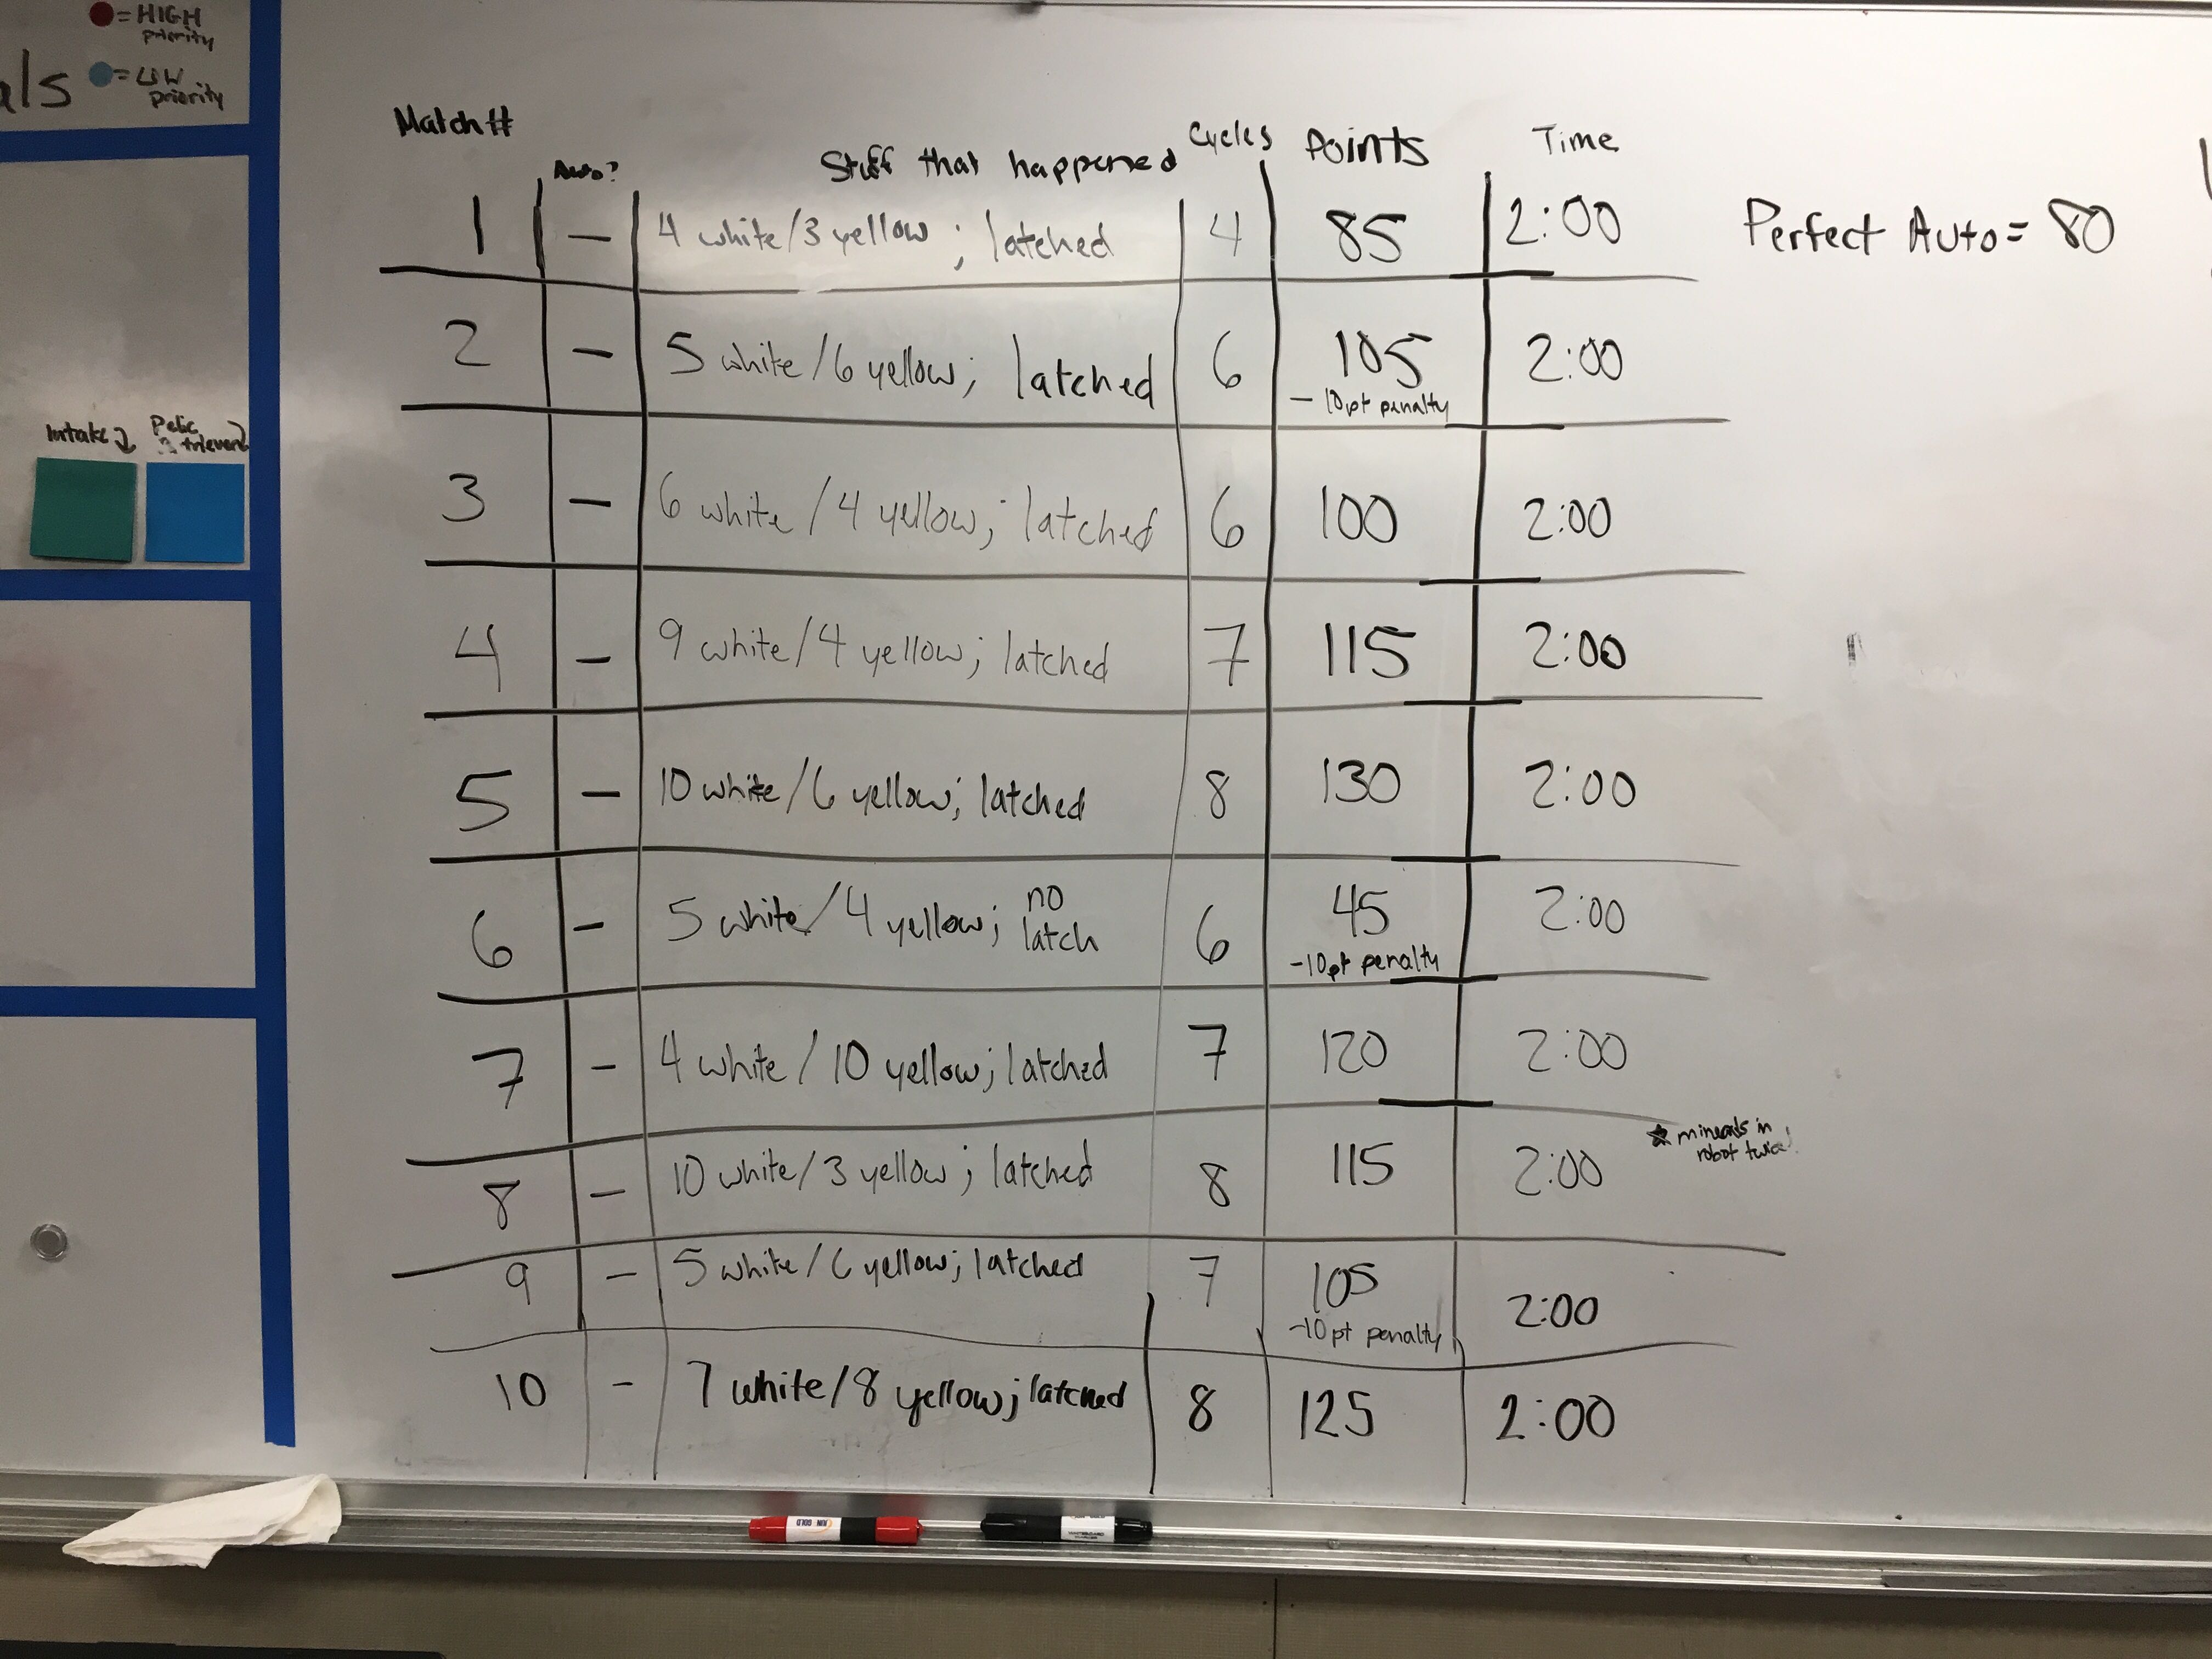
\includegraphics[width=.6 \textwidth]{23_02-04/images/IMG_1512.JPG}
    \caption{Score Keeping Chart}
    \label{fig:chart}
\end{figure}

\end{document}